\documentclass[11pt]{article}

% some definitions for the title page
\newcommand{\reporttitle}{New target volume delineation and PTV strategies to further
personalise radiotherapy}
\newcommand{\reportdescription}{Review of paper~\cite{personalised-PTV-strategies}}

% load some definitions and default packages
%%%%%%%%%%%%%%%%%%%%%%%%%%%%%%%%%%%%%%%%%
% University Assignment Title Page 
% LaTeX Template
% Version 1.0 (27/12/12)
%
% This template has been downloaded from:
% http://www.LaTeXTemplates.com
%
% Original author:
% WikiBooks (http://en.wikibooks.org/wiki/LaTeX/Title_Creation)
%
% License:
% CC BY-NC-SA 3.0 (http://creativecommons.org/licenses/by-nc-sa/3.0/)
% 
%
%%%%%%%%%%%%%%%%%%%%%%%%%%%%%%%%%%%%%%%%%
%----------------------------------------------------------------------------------------
%	PACKAGES AND OTHER DOCUMENT CONFIGURATIONS
%----------------------------------------------------------------------------------------
\usepackage[a4paper,hmargin=2.0cm,vmargin=1.0cm,includeheadfoot]{geometry}
\usepackage{textpos}

\usepackage[square,numbers]{natbib} % for bibliography
\usepackage[nottoc]{tocbibind} % Includes "References" in the table of contents
\bibliographystyle{unsrtnat}

\usepackage{tabularx,longtable,multirow,subfigure,caption}%hangcaption
\usepackage{fancyhdr} % page layout
\usepackage{url} % URLs
\usepackage[english]{babel}
\usepackage{amsmath}
\usepackage{graphicx}
\usepackage{scalerel}
\usepackage{dsfont}
\usepackage{epstopdf} % automatically replace .eps with .pdf in graphics
\usepackage{backref} % needed for citations
\usepackage{array}
\usepackage{latexsym}

\usepackage[pdftex,pagebackref,hypertexnames=false,colorlinks]{hyperref} % provide links in pdf
\usepackage{booktabs}
\usepackage{wrapfig}
\usepackage{caption}  % Required for \captionof
\usepackage{float} % for H option in figures
\usepackage{amssymb}
\usepackage{amsmath}
\usepackage{csquotes}
% \usepackage{subcaption} % causes a compilation error after changing back to natbib referencing... 

\hypersetup{pdftitle={},
  pdfsubject={}, 
  pdfauthor={},
  pdfkeywords={}, 
  pdfstartview=FitH,
  pdfpagemode={UseOutlines},% None, FullScreen, UseOutlines
  bookmarksnumbered=true, bookmarksopen=true, colorlinks,
    citecolor=black,%
    filecolor=black,%
    linkcolor=black,%
    urlcolor=black}

\usepackage[all]{hypcap}

%%%%%%%%%%%%%%%%%%%%%%%%%%%%%%%%%%%%%%%%%%%%%%%%%%%%%%%%%%%%%%%%%%%%%%%%%%%%%%%%
% LISTINGS ammendments
%%%%%%%%%%%%%%%%%%%%%%%%%%%%%%%%%%%%%%%%%%%%%%%%%%%%%%%%%%%%%%%%%%%%%%%%%%%%%%%%
\usepackage{listings}

\lstset
{ %Formatting for code in appendix
    language=Matlab,
    basicstyle=\footnotesize,
    % numbers=left,
    stepnumber=1,
    showstringspaces=false,
    tabsize=1,
    breaklines=true,
    breakatwhitespace=false,
    frame=single,
    columns=fullflexible,
    postbreak=\mbox{\textcolor{red}{$\hookrightarrow$}\space},
}

%\usepackage{color}
%\usepackage[tight,ugly]{units}
%\usepackage{float}
%\usepackage{tcolorbox}
%\usepackage[colorinlistoftodos]{todonotes}
% \usepackage{ntheorem}
% \theoremstyle{break}
% \newtheorem{lemma}{Lemma}
% \newtheorem{theorem}{Theorem}
% \newtheorem{remark}{Remark}
% \newtheorem{definition}{Definition}
% \newtheorem{proof}{Proof}


%%% Default fonts
\renewcommand*{\rmdefault}{bch}
\renewcommand*{\ttdefault}{cmtt}


%%% Default settings (page layout)
\setlength{\parindent}{0em}  % indentation of paragraph
\setlength{\parskip}{.3em}

% \setlength{\parindent}{0em}  % indentation of paragraph

\setlength{\headheight}{14.5pt}
\pagestyle{fancy}
\renewcommand{\chaptermark}[1]{\markboth{\chaptername\ \thechapter.\ #1}{}}
%\fancyhead[RO]{\sffamily \textbf{\thepage}} %Page no.in the right on even pages
%\fancyhead[LE]{\sffamily \textbf{\thepage}} %Page no. in the left on odd pages

\fancyfoot[ER,OL]{\thepage}%Page no. in the left on
%odd pages and on right on even pages
\fancyfoot[OC,EC]{\sffamily }
\renewcommand{\headrulewidth}{0.1pt}
\renewcommand{\footrulewidth}{0.1pt}
\captionsetup{margin=10pt,font=small,labelfont=bf}


%--- chapter heading

\def\@makechapterhead#1{%
  \vspace*{10\p@}%
  {\parindent \z@ \raggedright \sffamily
    \interlinepenalty\@M
    \Huge\bfseries \thechapter \space\space #1\par\nobreak
    \vskip 30\p@
  }}

%--- chapter heading

\def\@makechapterhead#1{%
  \vspace*{10\p@}%
  {\parindent \z@ \raggedright \sffamily
    %{\Large \MakeUppercase{\@chapapp} \space \thechapter}
    %\\
    %\hrulefill
    %\par\nobreak
    %\vskip 10\p@
    \interlinepenalty\@M
    \Huge\bfseries \thechapter \space\space #1\par\nobreak
    \vskip 30\p@
  }}

%---chapter heading for \chapter*  
\def\@makeschapterhead#1{%
  \vspace*{10\p@}%
  {\parindent \z@ \raggedright
    \sffamily
    \interlinepenalty\@M
    \Huge \bfseries  #1\par\nobreak
    \vskip 30\p@
  }}
\allowdisplaybreaks
% Here, you can define your own macros. Some examples are given below.

\newcommand{\R}[0]{\mathds{R}} % real numbers
\newcommand{\Z}[0]{\mathds{Z}} % integers
\newcommand{\N}[0]{\mathds{N}} % natural numbers
\newcommand{\C}[0]{\mathds{C}} % complex numbers
% \renewcommand{\vec}[1]{{\boldsymbol{{#1}}}} % vector
\newcommand{\mat}[1]{{\boldsymbol{{#1}}}} % matrix

\usepackage{pifont,mdframed}
\newenvironment{warning}
  {\par\begin{mdframed}[linewidth=1pt,linecolor=black]%
    \begin{list}{}{\leftmargin=1cm
                  \labelwidth=\leftmargin}\item[\Large\ding{43}]}
  {\end{list}\end{mdframed}\par}

\definecolor{lightgray}{gray}{0.9}

\begin{document}

% Include the title page
% Last modification: 2015-08-17 (Marc Deisenroth)
\begin{titlepage}

    \newcommand{\HRule}{\rule{\linewidth}{0.5mm}} % Defines a new command for the horizontal lines, change thickness here
    
    %----------------------------------------------------------------------------------------
    %	LOGO SECTION
    %----------------------------------------------------------------------------------------
    
    
\includegraphics[width = 4cm]{../figures/imperial.pdf}\\[0.5cm] 
    
    \center % Center everything on the page
     
    %----------------------------------------------------------------------------------------
    %	HEADING SECTIONS
    %----------------------------------------------------------------------------------------
    
    \textsc{\LARGE \reporttype}\\[1.5cm] 
    \textsc{\Large Department of Computing}\\[0.5cm] 
    \textsc{\large Imperial College of Science, Technology and Medicine}\\[0.5cm] 
    
    %----------------------------------------------------------------------------------------
    %	TITLE SECTION
    %----------------------------------------------------------------------------------------
    
    \HRule \\[0.4cm]
    { \huge \bfseries \reporttitle}\\ % Title of your document
    \HRule \\[1.5cm]
     
    %----------------------------------------------------------------------------------------
    %	AUTHOR SECTION
    %----------------------------------------------------------------------------------------
    
    \begin{minipage}{0.4\textwidth}
    \begin{flushleft} \large
    \emph{Author:}\\
    \reportauthor % Your name
    \end{flushleft}
    \end{minipage}
    ~
    \begin{minipage}{0.4\textwidth}
    \begin{flushright} \large
    \emph{Supervisor:} \\
    \supervisor % Supervisor's Name
    \end{flushright}
    \end{minipage}\\[4cm]
    
    
    
    
    %----------------------------------------------------------------------------------------
    
    
    %----------------------------------------------------------------------------------------
    %	DATE SECTION
    %----------------------------------------------------------------------------------------
    
    {\large \today} % Date, change the \today to a set date if you want to be precise
    
    
    \vfill % Fill the rest of the page with whitespace
    Submitted in partial fulfillment of the requirements for the \degreetype~of Imperial College London
    
    \end{titlepage}
    

\tableofcontents

\clearpage

\section{Summary}

In PTVs geometrical uncertainty is typically derived from a limited sample of patients, which conequently means that the resulting margins are not tailored to individual patients. Standard PTVs cannot account for arbitrary anisotrpic extensions (\ref{term:arbitrary-anisotropic-extensions}) of the target volume originalting from Delinieation uncertainty. Delineation uncertainty is currently estimated by measuring variations between contours produced by different observers (a limitation of current practice is that DU is only measured for samples of patients, whcih prevents margins from accounting for DU associated with each individual patient).

\subsection{Method}

\begin{enumerate}
    \item Firstly, delineate two contour sets; one which bounds all voxels believed to have a probability of belonging to the GTV of 1, while the second includes all voxels with a probability greater than 0.
    \item specify a PDF for the true GTV boundary position within the boundaries of the two countours
    \item Create a patient-specific PTV, designed to account for all systematic erros using this information along with measurements of the other systematic errors.
\end{enumerate}

This method alegedly produces smaller PTVs than the van Herk margin recipe (\ref{term:herk-margin-recipe})

\subsection{Type B delineation method}

\begin{figure}[H]
    \centering
    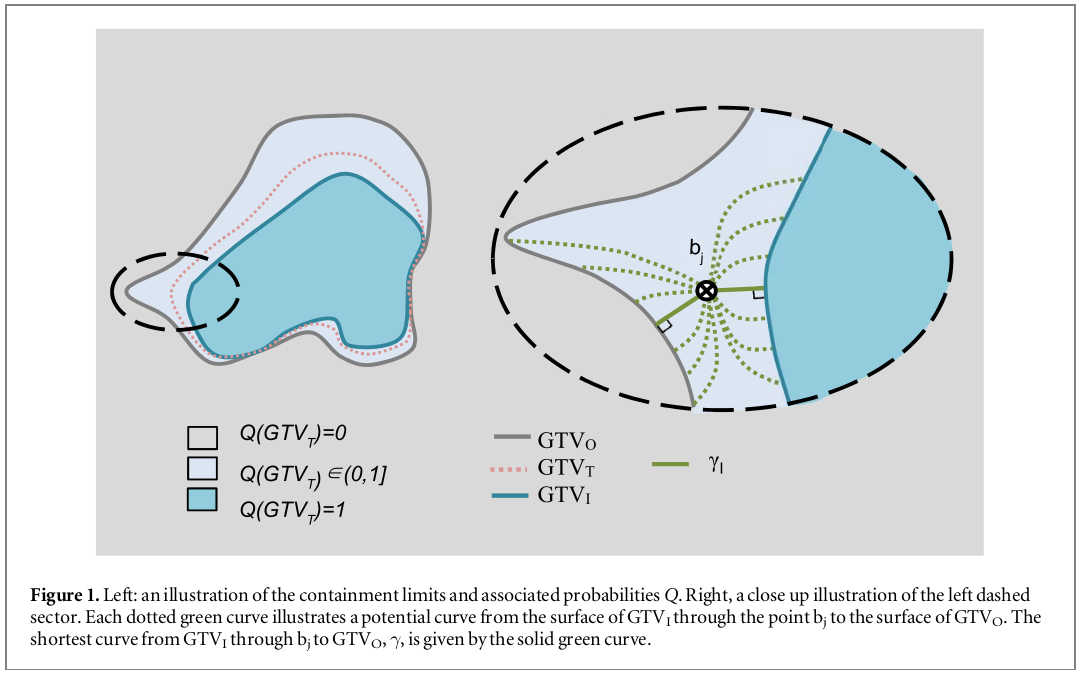
\includegraphics[width=\textwidth]{images/PDF-of-CTV.png}
    \caption{Illustration of certainty within a CTV}
    \label{fig:pdf-of-ctv}
\end{figure}

see original paper for formuals.

\subsection{Hand-wavy explination of the formulas}

From Figure\ref{fig:pdf-of-ctv} we have areas we are certian contain a tumour and an area that has a non-0 probability of it containing a tumour. 

We then obtain a distribution of uncertainty and find numerical values for $\varphi$ (the PDF). For each point we have a perpendicualr distance between the boundary of uncertainty and certainty (RHS of Figure \ref{fig:pdf-of-ctv}). We then convince ourselves that the intergral sums to 1.

We then incorporate systematic errors. See paper.

\section{Terminology}

\subsection{Arbitrary anisotropic extensions} \label{term:arbitrary-anisotropic-extensions}

Isotropic and anisotropic are terms that describe whether or not the properties of materials depend on direction. When a property is the same in all directions, the material is isotropic. When a property varies according to direction, the material is anisotropic. The terms come from the Greek isos (equal) and tropos (way). The an in “anisotropic” means “not.”~\cite{anisotropy}

\subsection{Herk Margin Recipe} \label{term:herk-margin-recipe}

\subsubsection{Will errors ever be zero?}

One might consider that because of modern developments in image-guided radiotherapy, it is possible to eliminate all geometrical errors and it may become safe to reduce the margin to zero. However, in my opinion, it is impossible to completely eliminate all geometrical errors. For instance, even if the treatment is completely accurate, there will still be uncertainties in GTV and CTV definition. Then, online systems for imageguided radiotherapy will not be perfectly accurate because of detection or observer errors in the imaging system. Then there will always be some delay between imaging and treatment leading to uncertainties because of short-term organ movement. Then, there will be limits on the accuracy of correction procedures. Finally, when using indirect methods for detection of the tumor position, there will still be the possibility of relative movement of the structure of reference and the tumor.~\cite{van-herk-margin-recipe}

\subsubsection{Herk Margin Recipe}

"The well-known Van Herk recipe for CTV-PTV margins~\cite{van-herk-margin-recipe2} assumes treatment uncertainties to be normally distributed and then studies the population histogram to ensure that 90\% of patients receive 95\% of the prescribed dose"~\cite{van-herk-margin-recipe3}~\cite{van-herk-margin-recipe2}

From~\cite{personalised-PTV-strategies} (paper in question)

\begin{equation}
    m = \alpha \Sigma + \beta \sqrt{\sigma^2 + \sigma^2_p} - \beta \sigma_p
\end{equation}

where $\Sigma$ is the systematic uncertainty, $\sigma$ is the random uncertainty, $\sigma_p$ is the measure of penumbra width (An area in which something exists to a lesser or uncertain degree (from google)) and $\alpha$ and $\beta$ denote the confidence level that the CTV is covered by a specified isodose for a given fraction of the patient population. And $m$ is the isotropic PTV-margin.

\subsubsection{Limitations}

With respect to DU, the MvHMR is limited by two assumptions. First, it assumes that the patient population is sufficiently homogeneous such that $\Sigma$ adequately represent the whole population even when measured in only a small sample of patients.
Second, the MvHMR assumes that all geometric uncertainties can be modelled by translations of the volume of interest (VOI). For target delineation, this implies that the clinician always delineates the target with the correct size and shape, but with errors simply being in its position. This is in conflict with the publications that show delineation error to be anisotropic, as described above. Therefore, the MvHMR is not designed to account for anisotropy which is known to exist for DU.

\printbibliography

\end{document}